\section{Análisis de outliers}

Antes de estudiar los coeficientes es necesario identificar, si es que los hay, aquellos países que pueden estar afectando a nuestro modelo en una manera no deseada por apartarse demasiado de los valores esperados.
Vamos a detectar outliers observando los gráficos de influencia (\textit{influence plots}) de los indicadores seleccionados.

Como se puede ver en el influence plot correspondiente al \textbf{Income Composition of Resources} (Figura \ref{fig:inf_icr}), no hay países que tengan valores medianamente altos de Leverage; es decir, no hay países que sean muy 'raros' en su valor de ICR. Algunos pueden tener un residuo studentizado medianamente alto, o una distancia de Cook no pequeña, pero al ser acompañados de Leverages bajos, no es necesario atenderlos.

\begin{figure}[H]
            \centering
             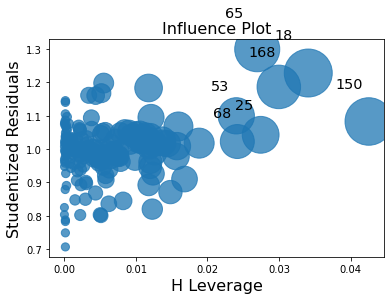
\includegraphics[scale = 0.5]{img/influ/icr.png}
             \caption{Influence plot correspondiente al ICR}
             \label{fig:inf_icr}
\end{figure}

Por otro lado, al analizar el gráfico relativo a \textbf{HIV/AIDS} podemos identificar un caso problemático.
El país con índice 155 (Suazilandia) exhibe a la vez valores altos en \textit{x}, en \textit{y} y en tamaño; es decir, tiene un valor 'raro' del indicador HIV/AIDS, es bastante distinto a lo predecible en su valor de Life Expectancy, y tiene mucho peso sobre el modelo.
Teniendo en cuenta este análisis, consideramos óptimo descartar la información que nos provee este país respecto a este indicador.
Más precisamente, reemplazamos su valor por la media. 
Con esta modificación el gráfico queda de la siguiente manera.

\begin{figure}[H]
            \centering
              \begin{subfigure}{0.45\linewidth}
                \centering
                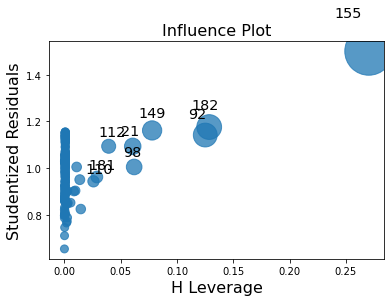
\includegraphics[width=\textwidth]{img/influ/hiv.png}
              \end{subfigure}
              \hfill
                \begin{subfigure}{0.45\linewidth}
                \centering
                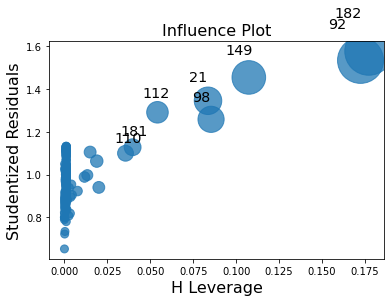
\includegraphics[width=\textwidth]{img/influ/hiv2.png}
              \end{subfigure}
             
               \caption{Influence plots para HIV/AIDS. A la izquierda, antes de modificar el valor de Swazilandia; a la derecha, después.}
               
               \label{fig:inf_hiv}
        \end{figure}
        
Continuando este análisis para \textbf{Diphtheria}, \textbf{BMI} y \textbf{percentage expenditure} no hallamos más outliers. En la Figura \ref{fig:inf_dift} se nota que los primeros dos manifiestan bajos valores sobre el eje \textit{x}. En el tercero también, excepto los países con índices 96 y 157. Estos países también exhiben una distancia de Cook considerable, pero no así la magnitud de los residuos studentizados. Por esto, no consideramos apropiado eliminar (o reemplazar el valor) de ninguno de estos elementos.  

\begin{figure}[H]
            \centering
              \begin{subfigure}{0.3\linewidth}
                \centering
                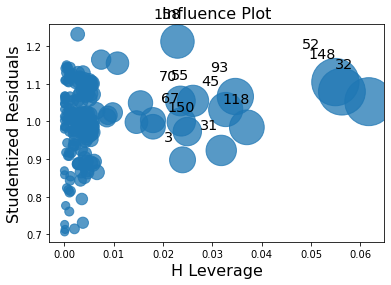
\includegraphics[width=\textwidth]{img/influ/difteria.png}
              \end{subfigure}
              \hfill
                \begin{subfigure}{0.3\linewidth}
                \centering
                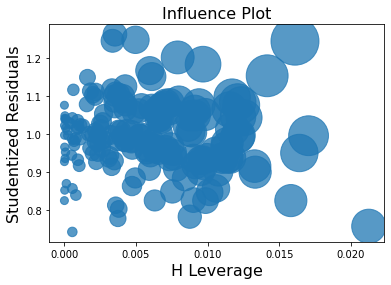
\includegraphics[width=\textwidth]{img/influ/bmi.png}
              \end{subfigure}
              \hfill
                \begin{subfigure}{0.3\linewidth}
                \centering
                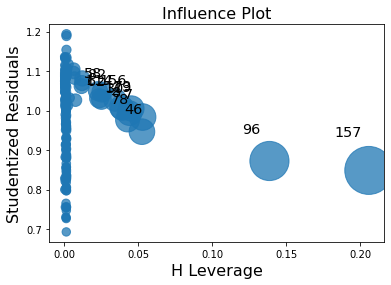
\includegraphics[width=\textwidth]{img/influ/percent_exp.png}
              \end{subfigure}
               \caption{Influence plots para Diphtheria (izq.), BMI (centro) y percentage expenditure (der.).}
               
               \label{fig:inf_dift}
        \end{figure}
        